\documentclass{article}
\usepackage{preamble}
\setlength\parskip{5pt}
\usetikzlibrary{math}



\makenoidxglossaries 

\newglossaryentry{AU}{
    name=astronomical unit,
    description={(AU) the unit of length defined as the average distance between Earth and the Sun; this distance is about \SI{1.5e8}{kilometers}}
}

\newglossaryentry{KIIIL}{
    name={Kepler's Third Law},
    description={the square of a planet's orbital period is directly proportional to the cube of the semimajor axis of its orbit}
}

\begin{document}
Astronomy \hfill Chapter 3: Orbits and Gravity \hfill Lecture Notes
\vspace{-5pt}

\hfill {\footnotesize Updated: \today}

\vspace{-1em}

\section*{The Laws of Planetary Motion}

\subsection*{Tycho Brahe's Observatory}

Recall: Ptolemy develops geocentric, complicated model for planetary motions in 140 AD

Recall: Copernicus published heliocentric (Sun-centered) hypothesis in 1549

Recall: Galileo observed Moon, Jupiter, Venus via telescope in 1609

Tycho Brahe (1546--1601): the last pre-telescopic observer in Europe

Made great recordings of positions of Sun and planets for 20 years

Noted that positions of planets varied from Ptolemy's (140 AD) model

Wanted better model than Ptolemy but unable to analyze data mathematically

1 year before death, hired young mathematician, Kepler
\vspace{5pt}

\hrule

\begin{problem}
    In what year was Tycho Brahe born? In what year did he die?
\end{problem}

\begin{problem}
    What was Tycho Brahe's greatest contribution to astronomy?
\end{problem}

\begin{problem}
    Did Brahe use a telescope in his observations?
\end{problem}

\begin{problem}
    What prevented Brahe from creating a better model of planetary motion than Ptolemy's ancient model?
\end{problem}

\begin{problem}
    Who did Brahe hire to analyze his data?
\end{problem}

\subsection*{Johannes Kepler}

Johannes Kepler (1571--1630): born into poor family in Germany

Studied theology at University of Tubingen

At Tubingen, learned about Copernican system, adopted heliocentric (Sun-centered) hypothesis 

Hired by Brahe to create model of planetary motion based on Brahe's data

Brahe restricted some resources to Kepler, wanted some glory of discovery

Brahe dies, Kepler gains full access to Brahe's data

\begin{problem}
    In what year was Johannes Kepler born? In what year did he die
\end{problem}

\begin{problem}
    Kepler studied \rule{2cm}{0.15mm} at the University of \rule{2cm}{0.15mm} .
\end{problem}

\begin{problem}
    What idea or system did Kepler encounter during his time in the university?
\end{problem}

\begin{problem}
    Who hired Kepler? For what purpose was Kepler hired?
\end{problem}

\begin{problem}
    What did Kepler inherit from Brahe?
\end{problem}

\clearpage

\subsection*{The First Two Laws of Planetary Motion}

Kepler wrote 3 laws of planetary motion.

orbit: the curved path of a planet around the Sun

Recall: Kepler inherits Brahe's mountain of observational data

Recall: Ptolemy's complex model contained only circles; 

Pythagoras said gods love circles

Kepler assumed circular orbits for planets. 

Brahe's data NOT in agreement with circular orbit

Kepler sees orbit of Mars is an ellipse (flattened circle)

\begin{figure}[h!]
    \centering

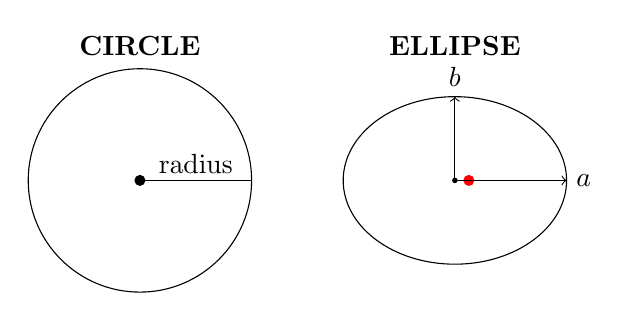
\begin{tikzpicture}
\tikzmath{
    \a = 2;
    \b = 1.5;
    \c = sqrt{\a^2 - \b^2};
}
\pgfplotsset{compat=1.11}
    \begin{axis}[
        width=3cm, height=3cm,
        axis line style={draw=none},
        ticks=none,
        axis lines=middle,
        ymin=-1, ymax=1,
        xmin=-1, xmax=1,
        clip=false,
    ]
        \draw (0,0) circle (2);
        \fill (0,0) circle (2pt);
        \draw (0,0) -- (2,0);
        \node at (1,0.3) {radius};
        \node at (0,2.4) {\textbf{CIRCLE}};
    \begin{scope}[xshift=4cm]
        \draw (0,0) ellipse ({\a} and {\b});
        \fill (0,0) circle (1pt);
        %\fill[red] (\c,0) circle (2pt);
        \fill[red] (-\c,0) circle (2pt);
        \draw[->] (0,0) -- (\a,0) node[right] {$a$};
        \draw[->] (0,0) -- (0,\b) node[above] {$b$};
        \node at (0,2.4) {\textbf{ELLIPSE}};
    \end{scope}
    \end{axis}
    \end{tikzpicture}
\end{figure}
\vspace{-1cm}

\begin{align*}
    a &= \text{semi major axis}\\
    b &= \text{semi minor axis}\\
\end{align*}

Kepler disagrees with Greek love for circles.

\begin{mdframed}[backgroundcolor=black!10]
    \textbf{Kepler’s First Law}: The orbit of each planet is an ellipse.
\end{mdframed}

The universe does not require only circles; it accepts the ellipse. 

\vspace{1em}
\hrule

\begin{problem}
    What is an orbit?
\end{problem}

\begin{problem}
At first, what did Kepler assume was the shape of a planet's orbit? Why did he assume this?
\end{problem}

\begin{problem}
    What made Kepler change his mind about his original assumption of the shape of orbits?
\end{problem}

\begin{problem}
    What is an ellipse?
\end{problem}

\begin{problem}
    What is Kepler's First Law of Planetary Motion?
\end{problem}



\clearpage
% \framebox{\textbf{Warm-Up}} Go to \href{https://openstax.org/books/astronomy-2e/pages/3-1-the-laws-of-planetary-motion}{OpenStax Astronomy Chapter 3}. What is Kepler's Second Law of planetary motion? Write your answer in your notebook.

\begin{mdframed}[backgroundcolor=black!10]
\textbf{Kepler's Second Law}: When closer to the Sun, the planet moves faster, and when farther away, it moves slower, but it sweeps out equal areas in an equal times.
\end{mdframed}

\begin{problem}
Kepler's Second Law of Motion
states that when a planet is closer to the Sun, it moves \rule{2cm}{0.15mm}, and when it's farther away, it
moves \rule{2cm}{0.15mm}, sweeping out equal areas in an equal times.
\end{problem}

\subsection*{Kepler's Third Law}

Planets closer to the Sun (e.g. Mercury, Venus) orbit the Sun in a short amount of time. Planets far away, (e.g., Neptune) take many years to orbit. 

Kepler wanted a mathematical relationship to calculate orbital periods.

orbital period ($P$): the time it takes a planet to travel once around the Sun

\gls{AU} (AU): average distance between Earth and Sun; 1 AU = \SI{1.5e8}{km}

Semimajor axis ($a$) is the average distance from a planet to the Sun.

\begin{mdframed}[backgroundcolor=black!10]
\gls{KIIIL} states that the orbital period squared is proportional to the semimajor axis cubed:
\vspace{-1em}

\begin{equation*}
    P^2 \propto a^3
\end{equation*}

If $P$ is expressed in units of years and $a$  in astronomical units (AU), then
\vspace{-1em}

\begin{equation*}
    P^2 = a^3
\end{equation*}

This law implies that the greater the distance between the Sun and the planet, the more time it will take the planet to orbit once around the Sun.
\end{mdframed}

\begin{example}
The distance from Mars to the Sun (Mars' semimajor axis) is \SI{1.52}{AU}. (Recall, for Earth it's \SI{1}{AU} by definition.) What is the orbital period of Mars in years?

\textit{Solution}

$a=1.52$. We want to find $P$. If

\begin{equation*}
    P^2 = a^3
\end{equation*}

then

\begin{equation*}
    P = \sqrt{a^3} = \sqrt{1.52^3} = \sqrt{1.52 \times 1.52 \times 1.52} = \SI{1.87}{years}
\end{equation*}
\end{example}

\begin{example}
What is the orbital period of an object with a semimajor axis of \SI{50}{AU} (50 times the Earth-Sun distance)?

\textit{Solution}

$a=50$ and, by Kepler's Third Law, $P^2 = a^3$. So, period is

\begin{equation*}
    P = \sqrt{a^3} = \sqrt{50^3} = \sqrt{50 \times 50 \times 50} = \SI{353}{years}
\end{equation*}
\end{example}

\begin{example}
What is the period of an asteroid with a semimajor axis of \SI{3}{AU}?

\begin{equation*}
    P = \sqrt{a^3} = \sqrt{3^3} = \sqrt{27} = \SI{5.2}{yr}
\end{equation*}
\end{example}

\clearpage
\begin{problem}
What is Kepler's Third Law of Motion?
\end{problem}

\begin{problem}
In Kepler's Third Law, what does the $P$ stand for? What units should be used?
\end{problem}

\begin{problem}
In Kepler's Third Law, what does the $a$ stand for? What units should be used?
\end{problem}

\begin{problem}
Jupiter has a semimajor axis of \SI{5.2}{AU}. What is its orbital period in years?
\end{problem}

\begin{figure}[h!]
\centering
\begin{tikzpicture}
\pgfplotsset{compat=1.11}
\def\ang{50}
\begin{axis}[
    width=18cm,height=18cm,
    axis line style={draw=none},
    ticks=none,
    xmin=-6,xmax=6,
    ymin=-6,ymax=6,
    clip=false,
    axis lines=middle
]
    \begin{scope}[xshift=-6cm]
        \clip (-0.1,-5) rectangle (10,5);
        \fill[orange] (0,0) circle (3pt);
        \draw[black!10] (0,0) circle (0.39);
        \draw[black!10] (0,0) circle (0.72);
        \draw[thick] (0,0) circle (1.00);
        \draw[black!50] (0,0) circle (1.52);
        \draw[black!50] (0,0) circle (5.20);
        \draw[black!50] (0,0) circle (9.54);
        \draw[->,thick] (0,0) -- (1,0) node[above left] {\SI{1}{AU}};
        \fill (1.52,0) circle (2pt) node[right=3pt] {Mars};
        \fill (5.2,0) circle (3pt) node[right=3pt] {Jupiter};
        \fill (9.54,0) circle (3pt) node [left=3pt] {Saturn};
    \end{scope}
\end{axis}
\end{tikzpicture}
\end{figure}

\begin{problem}
% Calculate orbital periods for the following semimajor axes (all in AU): 0.387, 0.723, 1.00, 1.52, 5.20, 9.54, 19.2, 30.1, 39.5
Go to \href{https://openstax.org/books/astronomy-2e/pages/3-4-orbits-in-the-solar-system}{OpenStax Ch.~3.4 Orbits in the Solar System} and find Table 3.2, which summarizes the semimajor axes in AU of the planets in the solar system. Use Kepler's 3rd Law $\left(P=\sqrt{a^3}\right)$ to calculate the orbital period in years of each planet. Confirm your results with the values for period in the table.
\end{problem}



\hrule
\clearpage  
\section*{Gravity}
Kepler: ``Planets move in ellipses around the Sun'' (1st law).

Isaac Newton: ``It's natural for objects to move in a staight line. Something must be bending the path of the planet." That something is gravity from the Sun.

\begin{mdframed}[backgroundcolor=black!10]
Newton realized that any two objects exert a gravitational force on each other. The Sun exerts a gravitational force on Earth, and vice versa. To calculate the exact amount of force exerted by Sun on a planet, we use Newton's Law of Universal Gravitation:
\begin{equation*}
    F = \frac{G m M}{r^2}\ .
\end{equation*}

Each quantity is summarized below

\begin{center}
    \begin{tabular}{cl|cl}
    \hline
    \textbf{Symbol} & \textbf{Quantity} & \textbf{SI Base Unit} & \textbf{Unit Symbol}  \\
    \hline\hline
    \rule{0pt}{2.5ex}
        $F$ & gravitational force between two masses & newton & N\\
        $G$ & gravitational constant & (\textit{see} $\rightarrow$) & \SI{}{N \cdot m^2/kg^2}\\
        $m$ & mass of planet & kilogram & kg\\
        $M$ & mass of Sun & kilogram & kg\\
        $r$ & distance between planet and Sun & meter & m\\
    \hline
    \end{tabular}
\end{center}

where
\vspace{-1em}

\begin{equation*}
    G = \SI{6.67e-11}{}\ .
\end{equation*}

Note that $r$ is like semimajor axis $a$.
\end{mdframed}

\begin{example}
What is the gravitational force exerted by the Sun on Earth? Use the values below.

\begin{center}
    \begin{tabular}{c|c|c}
        \textbf{Earth's mass} & \textbf{Sun's mass} & \textbf{Earth-to-Sun distance}\\
        \hline
        \SI{5.97e24}{kg} & \SI{1.99e30}{kg} & \SI{149e9}{m}\\
    \end{tabular}
\end{center}

\textit{Solution}

Substituting these values into Newton's Law of Gravitation leads to

\begin{equation*}
    F = \frac{G m M}{r^2} = \frac{\left(\SI{6.67e-11}{}\right) \left(\SI{5.97e24}{kg}\right) \left(\SI{1.99e30}{kg}\right)}{\left(\SI{149e9}{m}\right)^2}
    = \SI{3.6e22}{N}\ .
\end{equation*}

Therefore, according to Newton, an inward gravitational force of \SI{3.6e22}{N} (a humongous number!) from the Sun is needed to keep Earth bound in its orbit.
\end{example}

\clearpage
\begin{example}
What is the gravitational force of the Sun on Mercury? Use the values below.

\begin{center}
    \begin{tabular}{c|c|c}
        \textbf{Mercury's mass} & \textbf{Sun's mass} & \textbf{Mercury-to-Sun distance}\\
        \hline
        \SI{0.33e24}{kg} & \SI{1.99e30}{kg} & \SI{57.9e9}{m}\\
    \end{tabular}
\end{center}

\textit{Solution}

Mercury is way closer to the Sun than Earth is, so the gravitational force exerted by the Sun is expected to be greater. However, Mercury being less massive than Earth is a factor that decreases the Sun's gravitational force. We re-apply the Law of Gravitation, changing only two numbers:

\begin{equation*}
    F = \frac{G m M}{r^2} = \frac{\left(\SI{6.67e-11}{}\right) \left(\SI{0.330e24}{kg}\right) \left(\SI{1.99e30}{kg}\right)}{\left(\SI{57.9e9}{m}\right)^2}
    = \SI{1.3e22}{N}\ .
\end{equation*}

Therefore, even though Mercury is closer to the Sun, the Sun's gravitational force on Mercury is less than the Sun's gravitational force on Earth.
\end{example}
\hrule

\begin{problem}
What is the magnitude of the Sun's gravitational force on Venus? The mass of Venus is \SI{4.87e24}{kg} and its distance from the Sun (semimajor axis) is \SI{108.2e9}{m}. 
\end{problem}

\begin{problem}
    Calculate the magnitude of the Sun's gravitational force on Mars. The mass of Mars is \SI{0.642e24}{kg} and its distance from the Sun is \SI{228e9}{m}.
\end{problem}

\begin{problem}
    Calculate the magnitude of the Sun's gravitational force on Jupiter. The mass of Jupiter is \SI{1989e24}{kg} and its distance from the Sun is \SI{778.5e9}{m}.
\end{problem}

\begin{problem}
    Calculate the magnitude of the Sun's gravitational force on Saturn. The mass of Saturn is \SI{568e24}{kg} and its distance from the Sun is \SI{1432e9}{m}.
\end{problem}
\hrule

\clearpage
\begin{mdframed}[backgroundcolor=black!10]
Let $F_0 = \SI{3.6e22}{N}$ be the Sun's gravitational force on Earth. We can compare how the gravitational force by the Sun on another planet compares $F_0$ by using

\begin{equation*}
    \frac{F}{F_0} = \frac{\left(\frac{m}{5.97}\right)}{a^2}\ .
\end{equation*}

\begin{center}
    \begin{tabular}{cl|cl}
    \hline
    \textbf{Symbol} & \textbf{Quantity} & \textbf{Unit} & \textbf{Unit Symbol}  \\
    \hline\hline
    \rule{0pt}{2.5ex}
        $m$ & mass of planet & $10^{24}$ kilogram & $10^{24}\,\text{kg}$\\
        $a$ & distance between planet and Sun & astronomical units & AU\\
    \hline
    \end{tabular}
\end{center}

Note: $m$ and $a$ \textit{must} be in the units specified in the table. The above equation tells us how many times greater (or less than) the gravitational force by the Sun on the planet is compared to $F_0$. 
\vspace{-1em}

\begin{align*}
    \text{If } \frac{F}{F_0} < 1\ , \text{ then Sun's force on planet} < \text{Sun's force on Earth}\\[1ex]
    \text{If } \frac{F}{F_0} > 1\ , \text{ then Sun's force on planet} > \text{Sun's force on Earth} 
\end{align*}
\end{mdframed}

\begin{example}
How does the Sun's gravitational force on Mercury compare to that on Earth?

\textit{Solution}

As we saw in the prevous example, in units of $10^{24}\,$kg, Mercury's mass is $m=0.33$. According to Table 3.2 in \href{https://openstax.org/books/astronomy-2e/pages/3-4-orbits-in-the-solar-system}{OpenStax 3.4 Orbits in the Solar System}, Mercury's semimajor axis is $a = 0.39$. Therefore, 

\begin{equation*}
    \frac{F}{F_0} = \frac{\left(\frac{m}{5.97}\right)}{a^2} = \frac{\left(\frac{0.33}{5.97}\right)}{0.39^2} = 0.36\ ,
\end{equation*}

which is $<1$. Therefore, the Sun's gravitational force on Mercury is less than the Sun's force on Earth. Specifically, it's only 0.36 times the Sun's force on Earth.
\end{example}

\hrule

\begin{mdframed}[backgroundcolor=red!20]
For the remaining problems below, please see Table 3.2 in OpenStax Ch.~3.4 (\href{https://openstax.org/books/astronomy-2e/pages/3-4-orbits-in-the-solar-system}{click here}) for the semimajor axis data, and see the NASA Planetary Fact Sheet (\href{https://nssdc.gsfc.nasa.gov/planetary/factsheet/}{click here}) for planetary mass data.
\end{mdframed}

\begin{problem}
How does the Sun's gravitational force on \textbf{Venus} compare to the Sun's force on Earth? 
\end{problem}

\begin{problem}
How does the Sun's gravitational force on \textbf{Mars} compare to the Sun's force on Earth? 
\end{problem}

\begin{problem}
How does the Sun's gravitational force on \textbf{Jupiter} compare to the Sun's force on Earth? 
\end{problem}

\begin{problem}
How does the Sun's gravitational force on \textbf{Saturn} compare to the Sun's force on Earth? 
\end{problem}

\begin{problem}
How does the Sun's gravitational force on \textbf{Neptune} compare to the Sun's force on Earth? 
\end{problem}

% \begin{problem}
% Compare the Sun's gravitational force on each planet after Earth to the Sun's force on Earth. Planetary mass data is available at NASA's ``Planetary Fact Sheet'' (\href{https://nssdc.gsfc.nasa.gov/planetary/factsheet/}{click here}) and semimajor axis data is available in Table 3.2 in OpenStax Chapter 3.4: Orbits in the Solar System (\href{https://openstax.org/books/astronomy-2e/pages/3-4-orbits-in-the-solar-system}{click here}).
% \end{problem}

% \clearpage
\printnoidxglossaries





\end{document}